Tras reconocer los diferentes conceptos para la comprensión de la problemática mencionado en la \textbf{Sección \ref{sec:Conceptos}} y las relaciones que existen entre ellos, es que se realiza un diagrama de clases (ver \textbf{Figura \ref{fig: Diagrama_Clases}}) para representar el Modelo de Datos. Es por ello que a continuación se procede a detallar brevemente cada clase que compone el diagrama:

\begin{figure}[htb]
    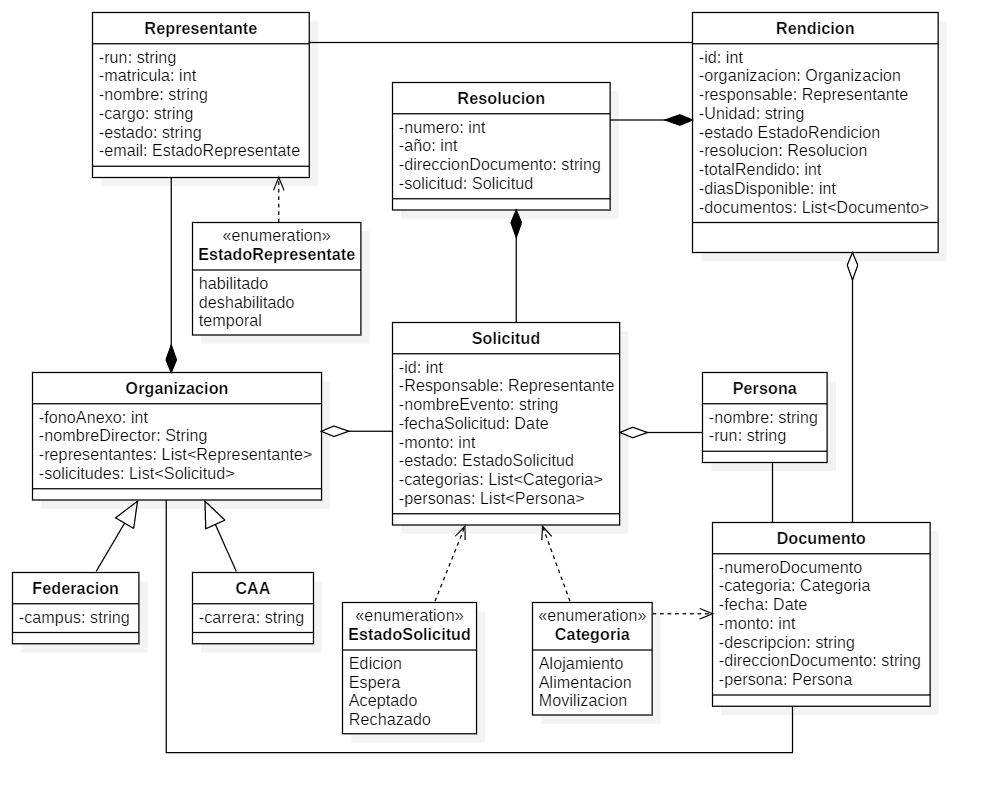
\includegraphics[width=\textwidth]{Imagenes/Diagrama_general_clases.png}
    \caption{\label{fig: Diagrama_Clases}Diagrama de clases que detalla el Modelo de Datos.}
\end{figure}

\begin{itemize}
    \item Solicitud: Representa la solicitud de un Fondo por Rendir por parte de la OE interesada.
    \item Persona: Representa los datos de los participantes de un evento (en caso de que el fondo solicitado sea para una o más personas) y son guardados en un listado en la clase Solicitud.
    \item Resolución: Representa la RU que acepta la solicitud y que es emitida por la Casa de estudio. Principalmente contiene atributos tales como el número de RU y el año de emisión.
    \item Rendición: Representa la declaración de gastos que se incurrieron en un evento solicitado por la OE. Principalmente contiene los datos de la organización, representante, el número de RU y un listado de documentos que contienen los datos de una boleta y/o factura. 
    \item Documento: Representa los datos que contiene una boleta y/o factura, los cuales son guardados en una lista en la clase Rendición.
    \item Organización: Representa los datos que contiene una OE de forma general. Presenta atributos tales como nombre del director a quien va dirigida las Solicitudes que realiza la OE, un listado de los Representantes y un listado de Solicitudes realizadas, entre otros.
    \item Federación: Representa a un usuario de tipo Federación y hereda de la clase \textbf{Organización}, por lo que también posee atributos que identifican a una organización. Además, contiene un atributo en específico que es campus al cual representa la Federación.
    \item CAA: Representa a un usuario de tipo CAA y hereda de la clase \textbf{Organización}, por lo que también tiene atributos que identifican a una organización. A diferencia de la clase Federación, esta clase contiene el atributo carrera para indicar de dónde proviene este tipo de OE.
    \item Representante: Especifica a uno de los Representantes que pertenece a la organización, el cual puede ser de dos tipos: presidente(a) o Secretario(a) de finanzas. Estos se encuentran en una lista que se encuentra en la clase Organización.
\end{itemize}


%Dado a que parte de la propuesta de solución corresponde al desarrollo de un sistema a través del cual las diferentes OE puedan utilizar para confeccionar la Rendición de un Fondo por Rendir y decir cuál es el óptimo monto que se ajusta al monto solicitado, es que se utiliza un algoritmo el cual ayuda a obtenerlo. Lo anterior interactúa con ciertas clases en específico las cuales son Documento y Rendición.
